\chapter{Majoron Decay Search}
To search for evidence of Majoron decays of $^{130}$Te, which deposit energy in CUORE's detectors with energies ranging up to the 2528 keV Q-value of $^{130}$Te as shown in \autoref{fig:Majoron Spectrum}, a precise understanding of the energy spectrum measured by CUORE is needed.
In essence, this search is purely a comparison of a $H_0$ hypothesis of physics without a Majoron contribution in favor of an $H_1$ hypothesis that includes Majoron decay.
However, constructing a ``true" $H_0$ model is not a trivial task, as it contains over 60 components in a background model for CUORE, all of which are fitted simultaneously.
In the worst-case scenario, an incorrect model could by happenstance be a good fit to the data; therefore, considerable work is undertaken to properly understand and characterize the components of the background model in CUORE.

\section{Background Sources in CUORE}
As discussed in \autoref{ssec:Parts Selection and Cleaning} and \autoref{ssec:Cryostat_Radiopurity}, there are multiple backgrounds that need to be considered when understanding the energy spectrum measured by the detectors.
These background come from radioactive contaminations in the cryostat components of CUORE and from external sources such as muons.
From the experience gained in CUORE-0, where a 57-component fit was performed to describe the energy spectrum observed \cite{Alduino:2016vtd}.
As CUORE-0 utilized a CUORE-like tower with the same cleaning and fabrication, the radioactive sources on the tower structures are expected to be the same in CUORE.
However, with the new cyrostat used for CUORE, the backgrounds due to the rest of the cryostat will differ from those in CUORE-0.

\subsection*{Source Reconstruction}
To perform a fit to the data, compiling a list of every component in CUORE with every contamination would be the most straightforward approach.
However, due to limited statistics in CUORE data, many of these sources are indistinguishable from one another, as shown in \autoref{fig:degenerate_sources}.
To solve this issue, these sources with ``degenerate" spectra are combined in the analysis and are combined into the same source in the fit.
In this way, much of the complexity of the fit can be reduced


\begin{figure}[htbp]
    \centering
    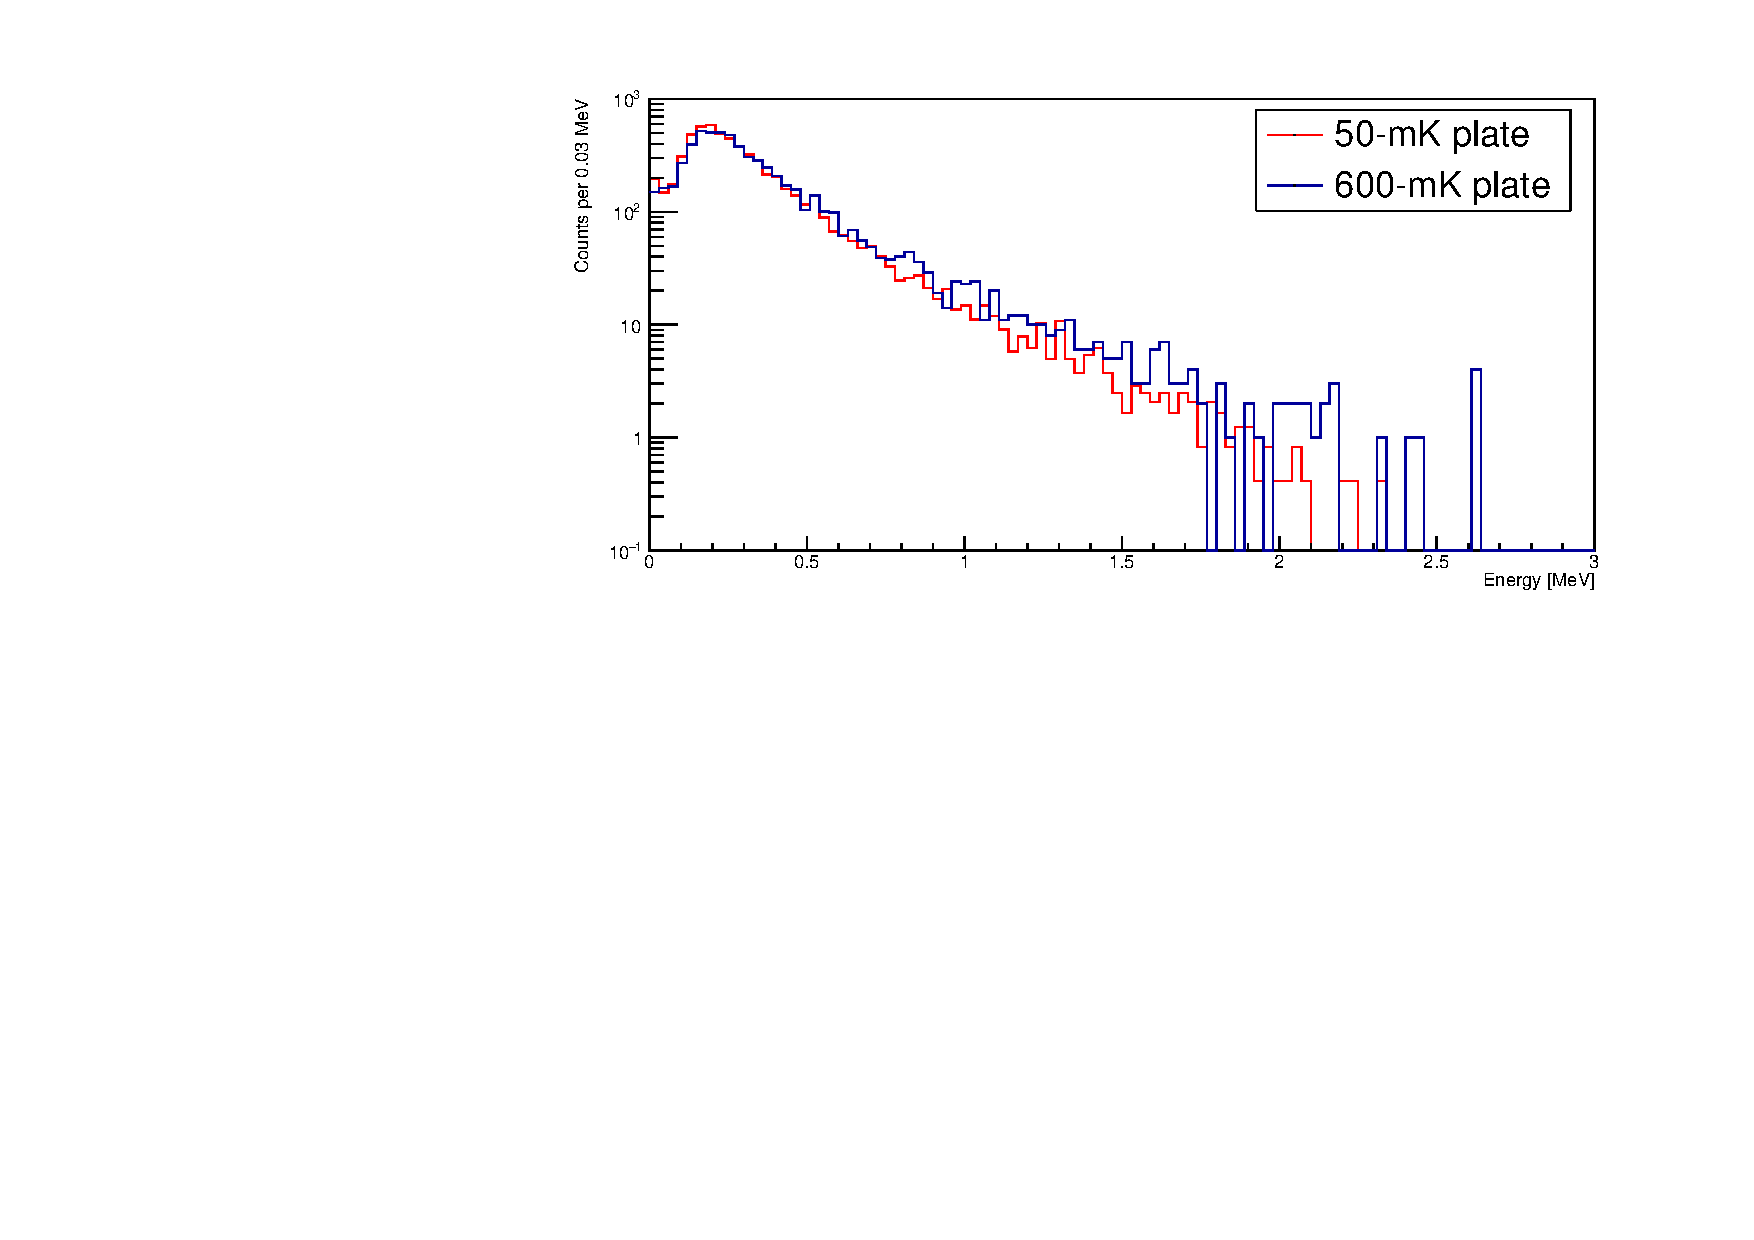
\includegraphics[width=0.8\linewidth]{Figures/th232_copper_plates.pdf}
    \caption[Simulated rates from a $^{232}$Th source on the 50-mK and 600-mK plates.]
    {Simulated rates from a $^{232}$Th source on the 50-mK and 600-mK plates.
    With limited statistics, the spectra of the two are degenerate.}
    \label{fig:degenerate_sources}
\end{figure}

\section{Markov Chain Monte Carlo}
\label{sec:MCMC}
Performing a simultaneous fit of $60+$ spectra is a non-trivial challenge, particularly as each component to the fit a
\subsection*{JAGS Analysis Software}
To perform this fit, we use a program called Just Another Gibbs Sampler (JAGS)\footnote{http://mcmc-jags.sourceforge.net/}.

describe how MCMC works exactly. Why does it give proper results? How should it be done properly
To perform a search for a spectrum-based rare event, it 

\section{Majoron Analysis}
When fitting the data with JAGS, the spectrum is split into two main components: the \Mone~spectrum, the \Mtwo~spectrum, and the summed \Msum~spectrum. This is done as the signal events from a Majoron search mostly deposit energy into a single crystal, as is typical of events originating from the bulk of the crystal volume, whereas many other sources that are external to a crystal or on the surface have a much higher probability of depositing energy into more than one crystal. Higher multiplicity spectra are not used, except for identifying the contribution of muons to the background, as they do not add significant information to the fit for other sources. For the fit, each of the possible Majoron spectral indices are considered independently and are shown for each multiplicity in \autoref{fig:SpectralIndicesM1Fit} and \autoref{fig:SpectralIndicesM2Fit}.


\begin{figure}[htbp]
\centering
\begin{subfigure}[t]{0.49\textwidth}
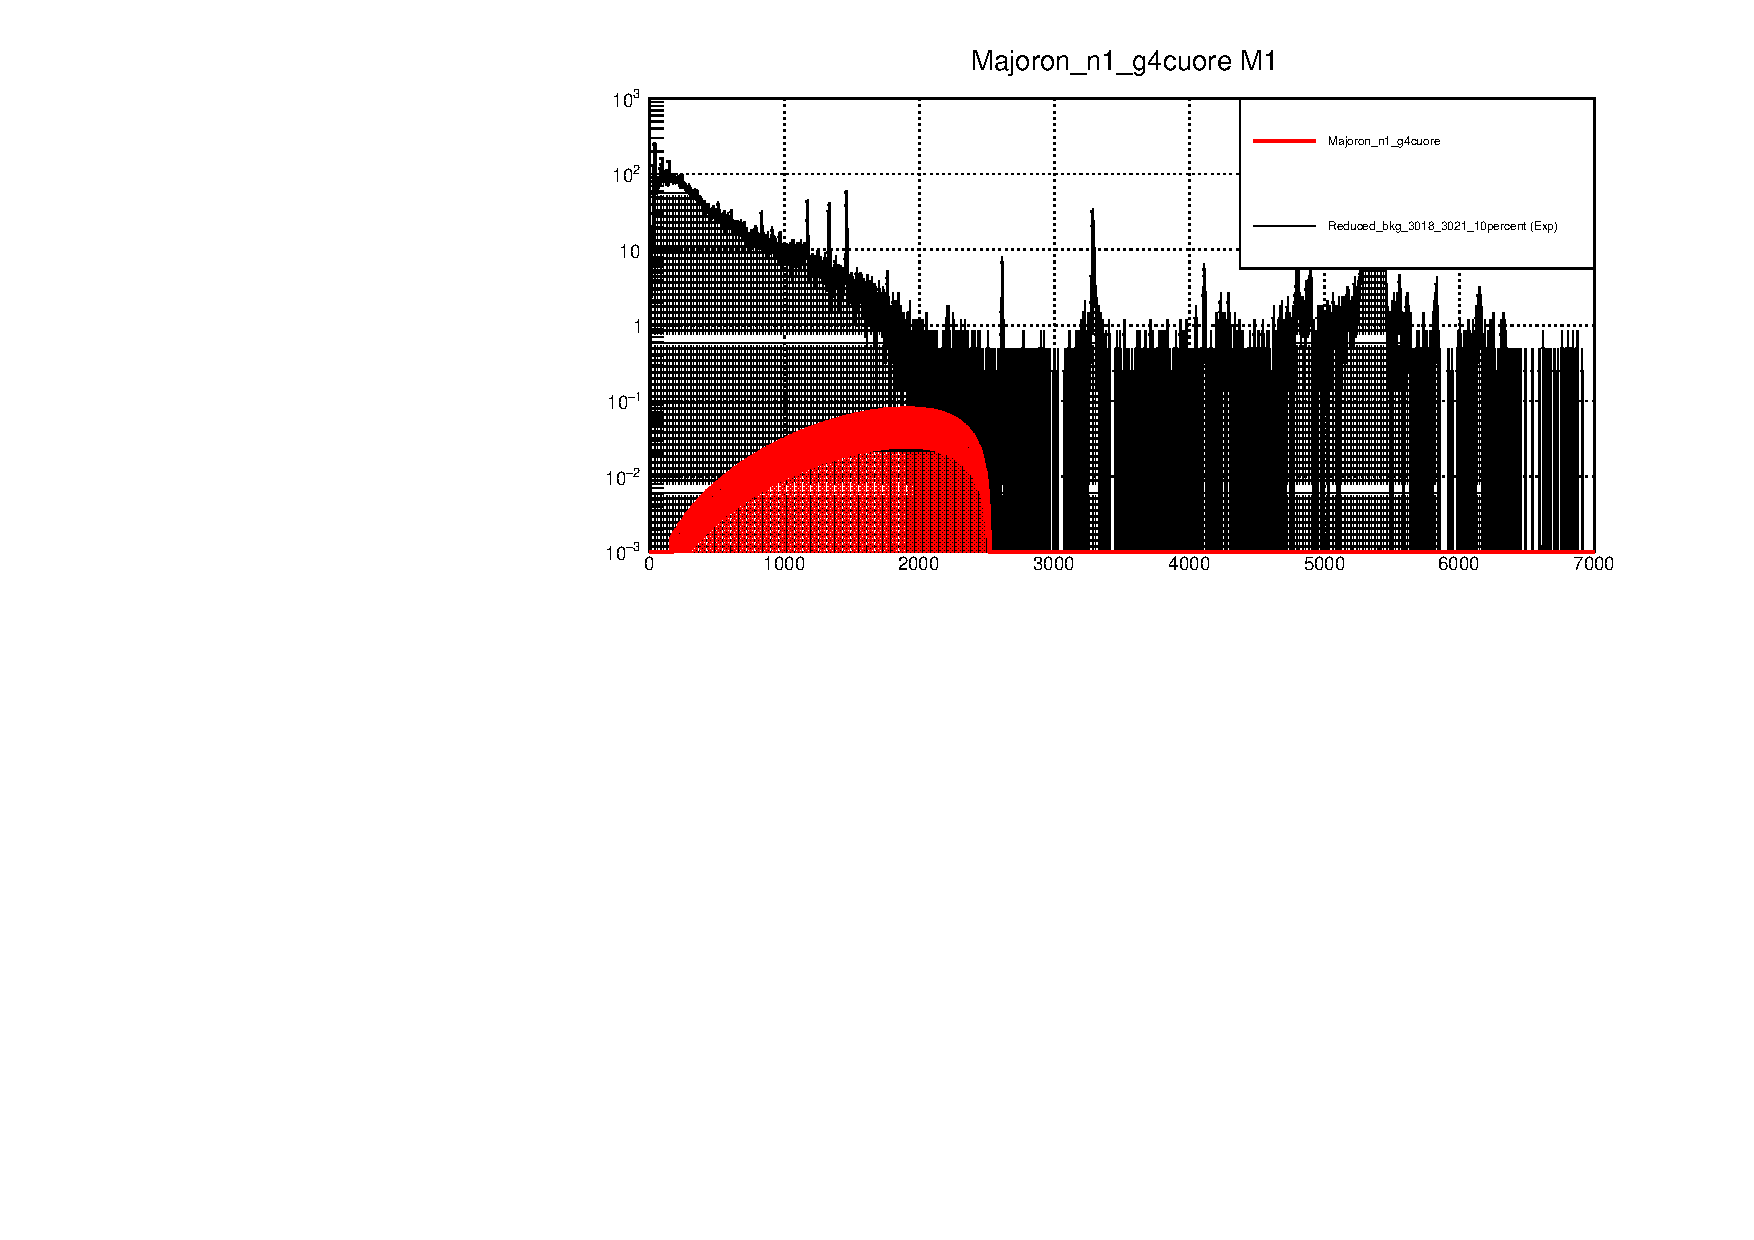
\includegraphics[width=0.9\textwidth]{Figures/Majoron_n1_g4cuore.pdf}
\end{subfigure}
\qquad
\begin{subfigure}[t]{0.49\textwidth}
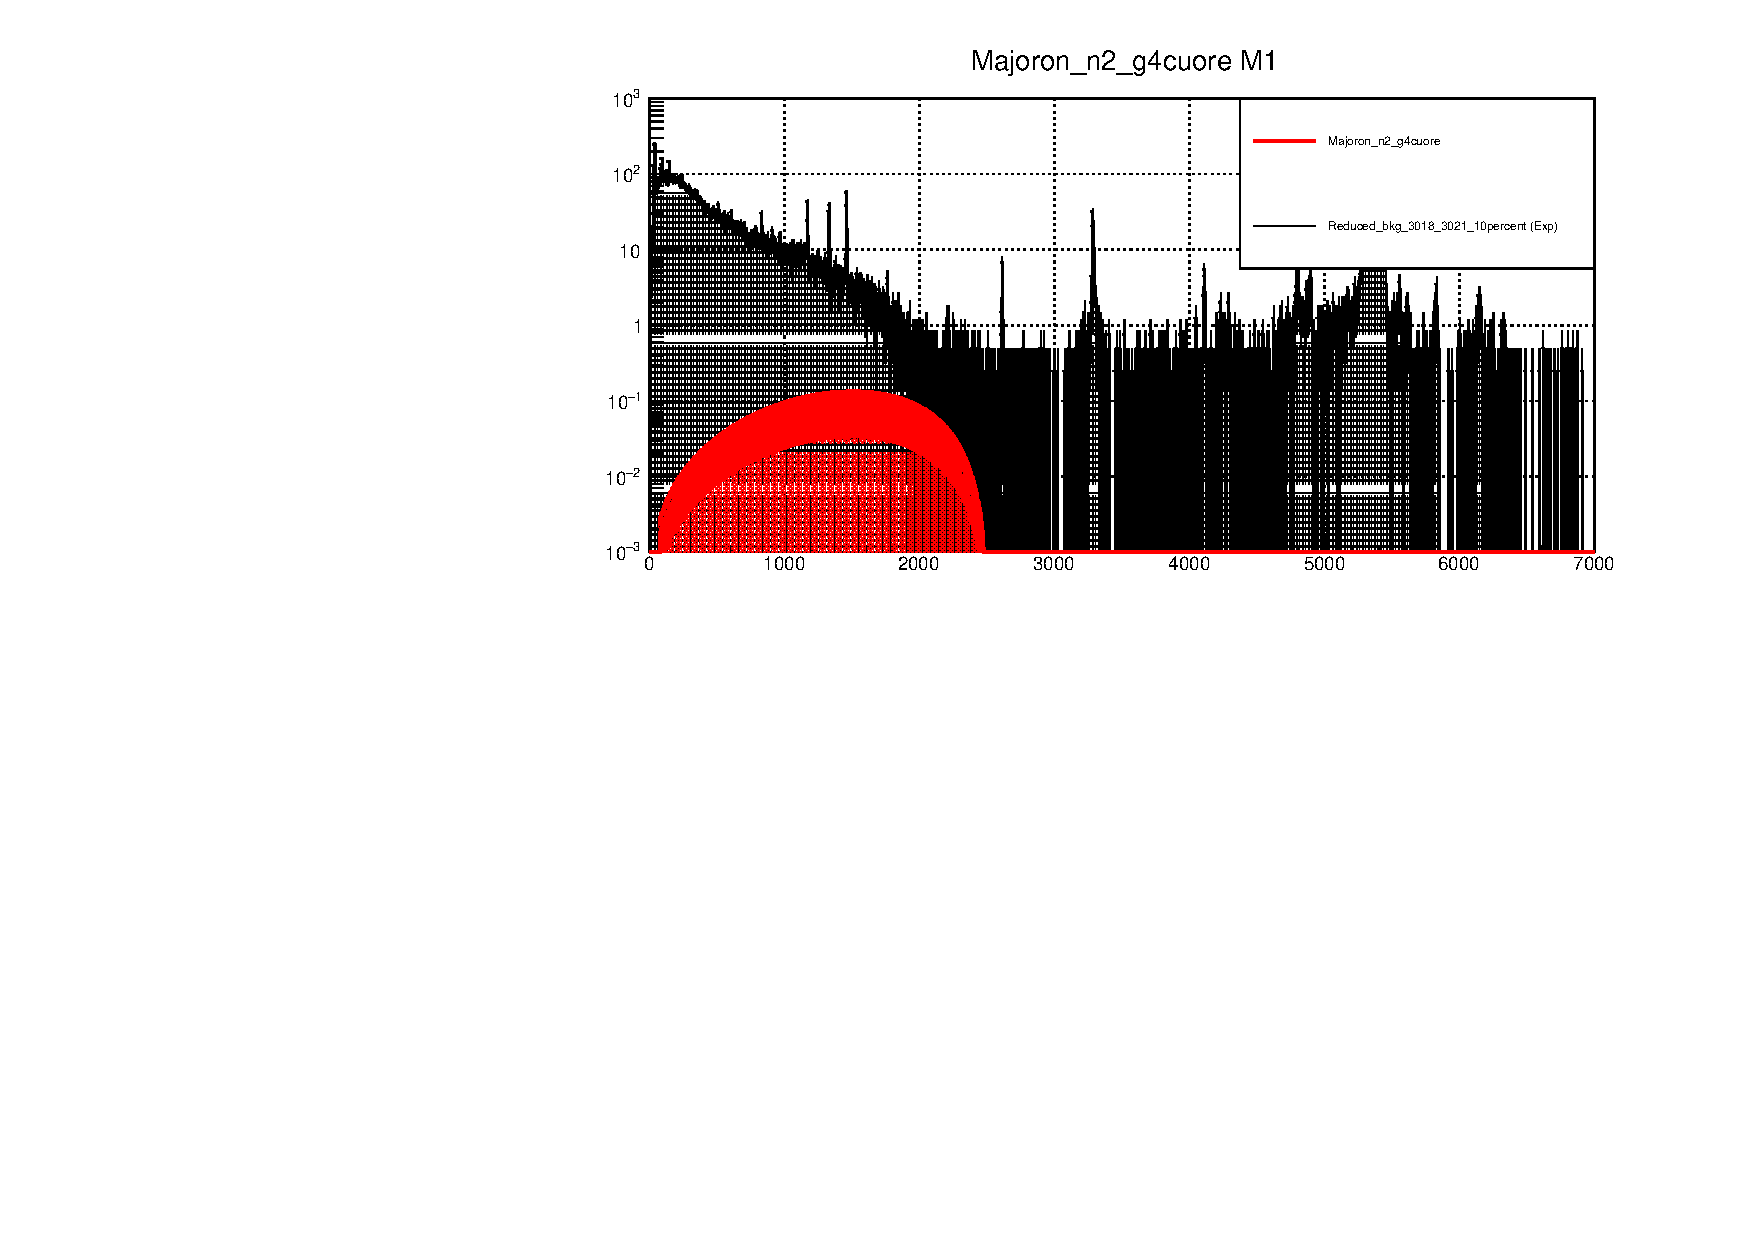
\includegraphics[width=0.9\textwidth]{Figures/Majoron_n2_g4cuore.pdf}
\end{subfigure}
\qquad
\begin{subfigure}[t]{0.49\linewidth}
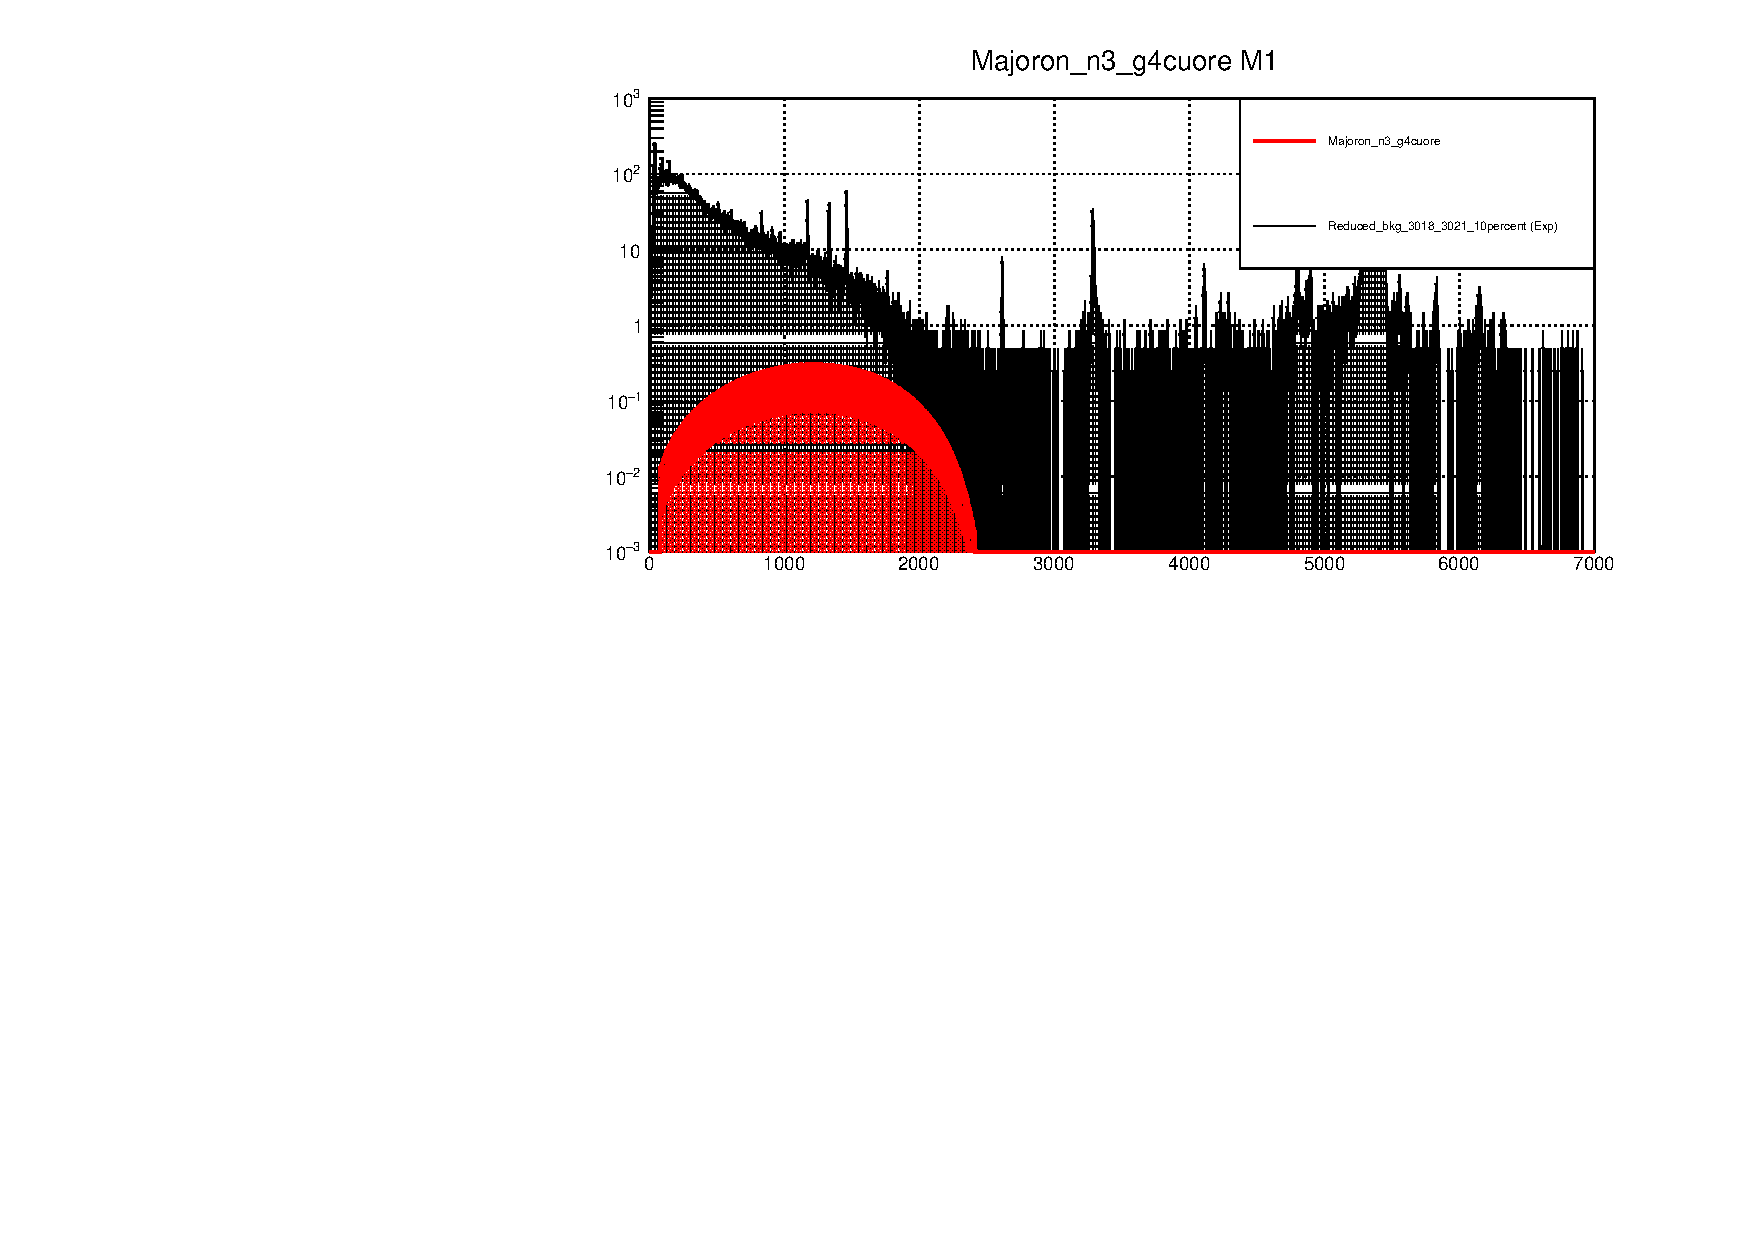
\includegraphics[width=0.9\textwidth]{Figures/Majoron_n3_g4cuore.pdf}
\end{subfigure}
\qquad
\begin{subfigure}[t]{0.49\linewidth}
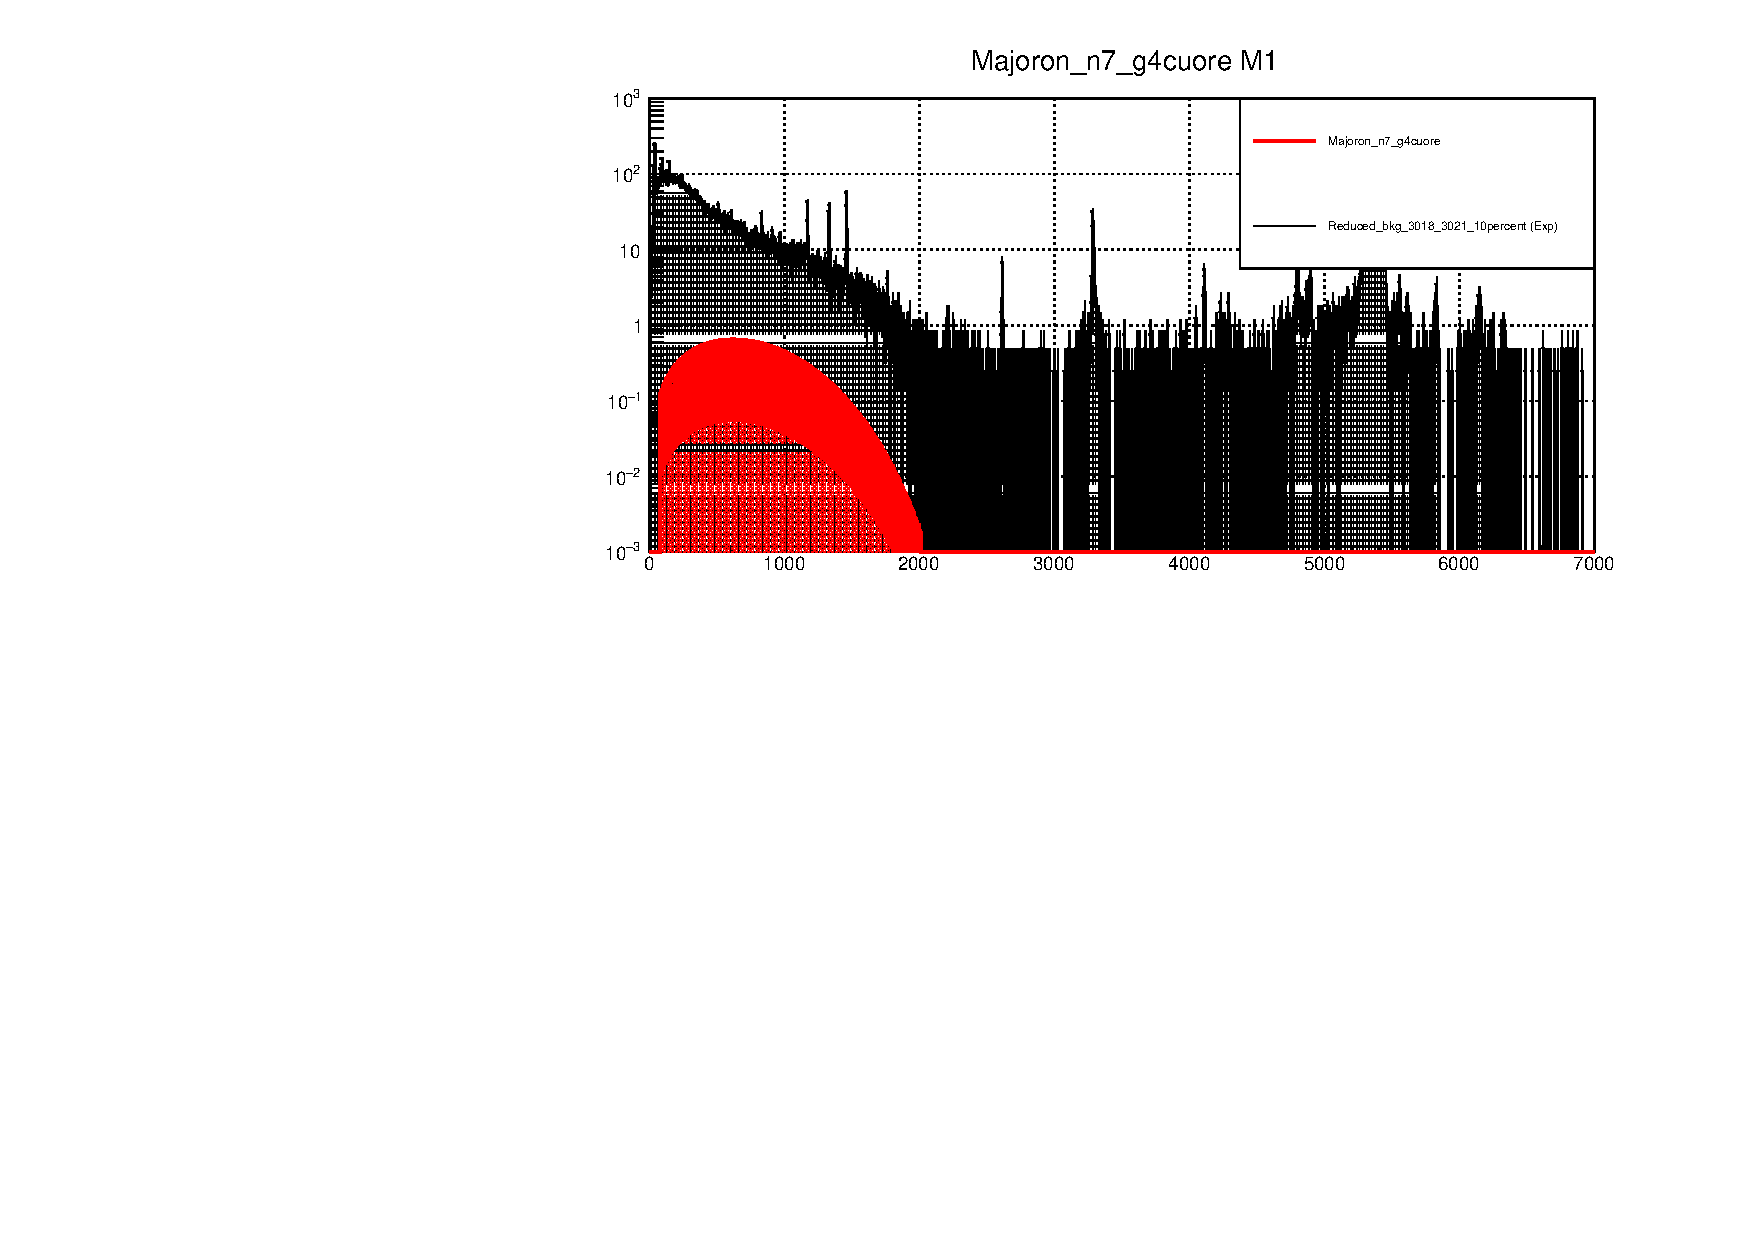
\includegraphics[width=0.9\textwidth]{Figures/Majoron_n7_g4cuore.pdf}
\end{subfigure}
\caption[The fitted contribution of Majoron decays for the different spectral indices in the \Mone~ spectrum.]{The fitted contribution of Majoron decays for the different spectral indices in the \Mone~ spectrum.}
\label{fig:SpectralIndicesM1Fit}
\end{figure}

\begin{figure}[htbp]
\centering
\begin{subfigure}[t]{0.49\textwidth}
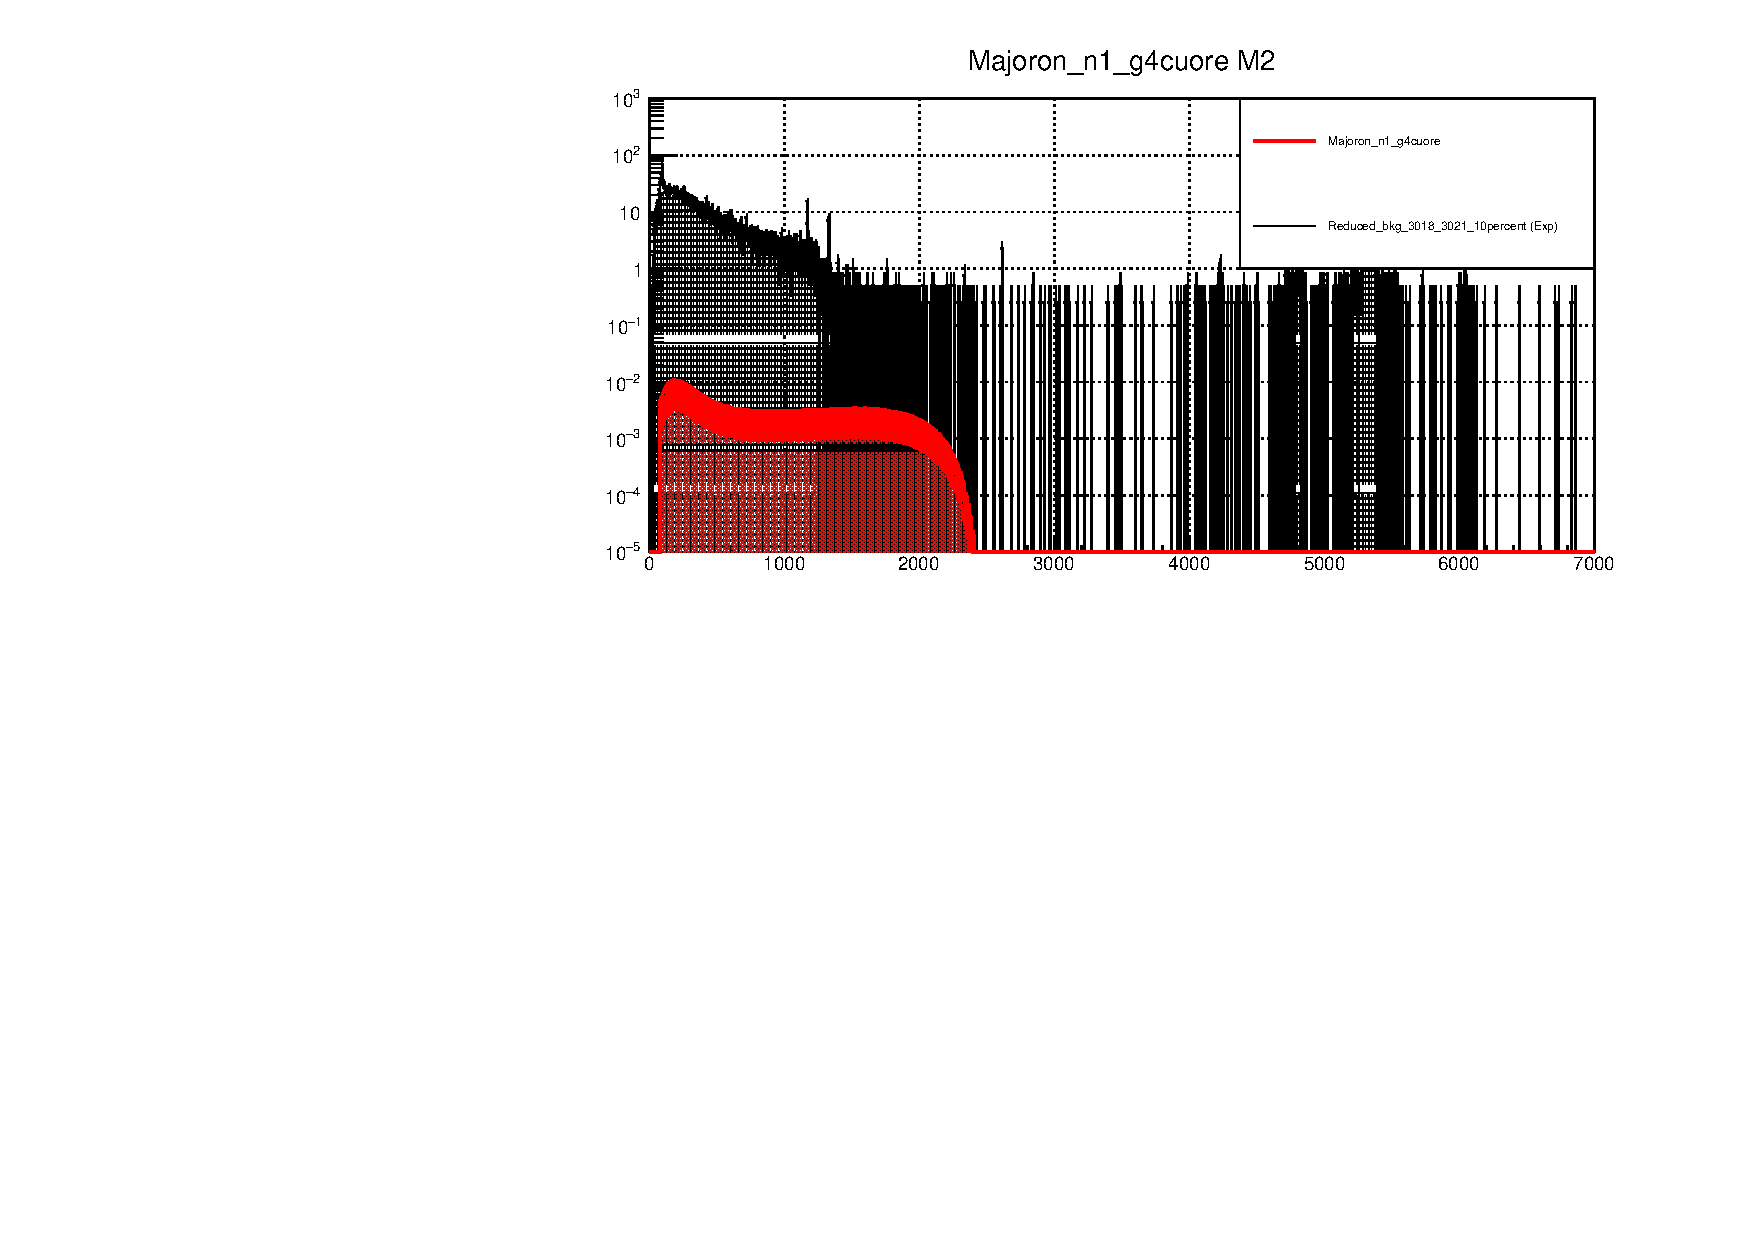
\includegraphics[width=0.9\textwidth]{Figures/Majoron_n1_g4cuore_M2.pdf}
\end{subfigure}
\qquad
\begin{subfigure}[t]{0.49\textwidth}
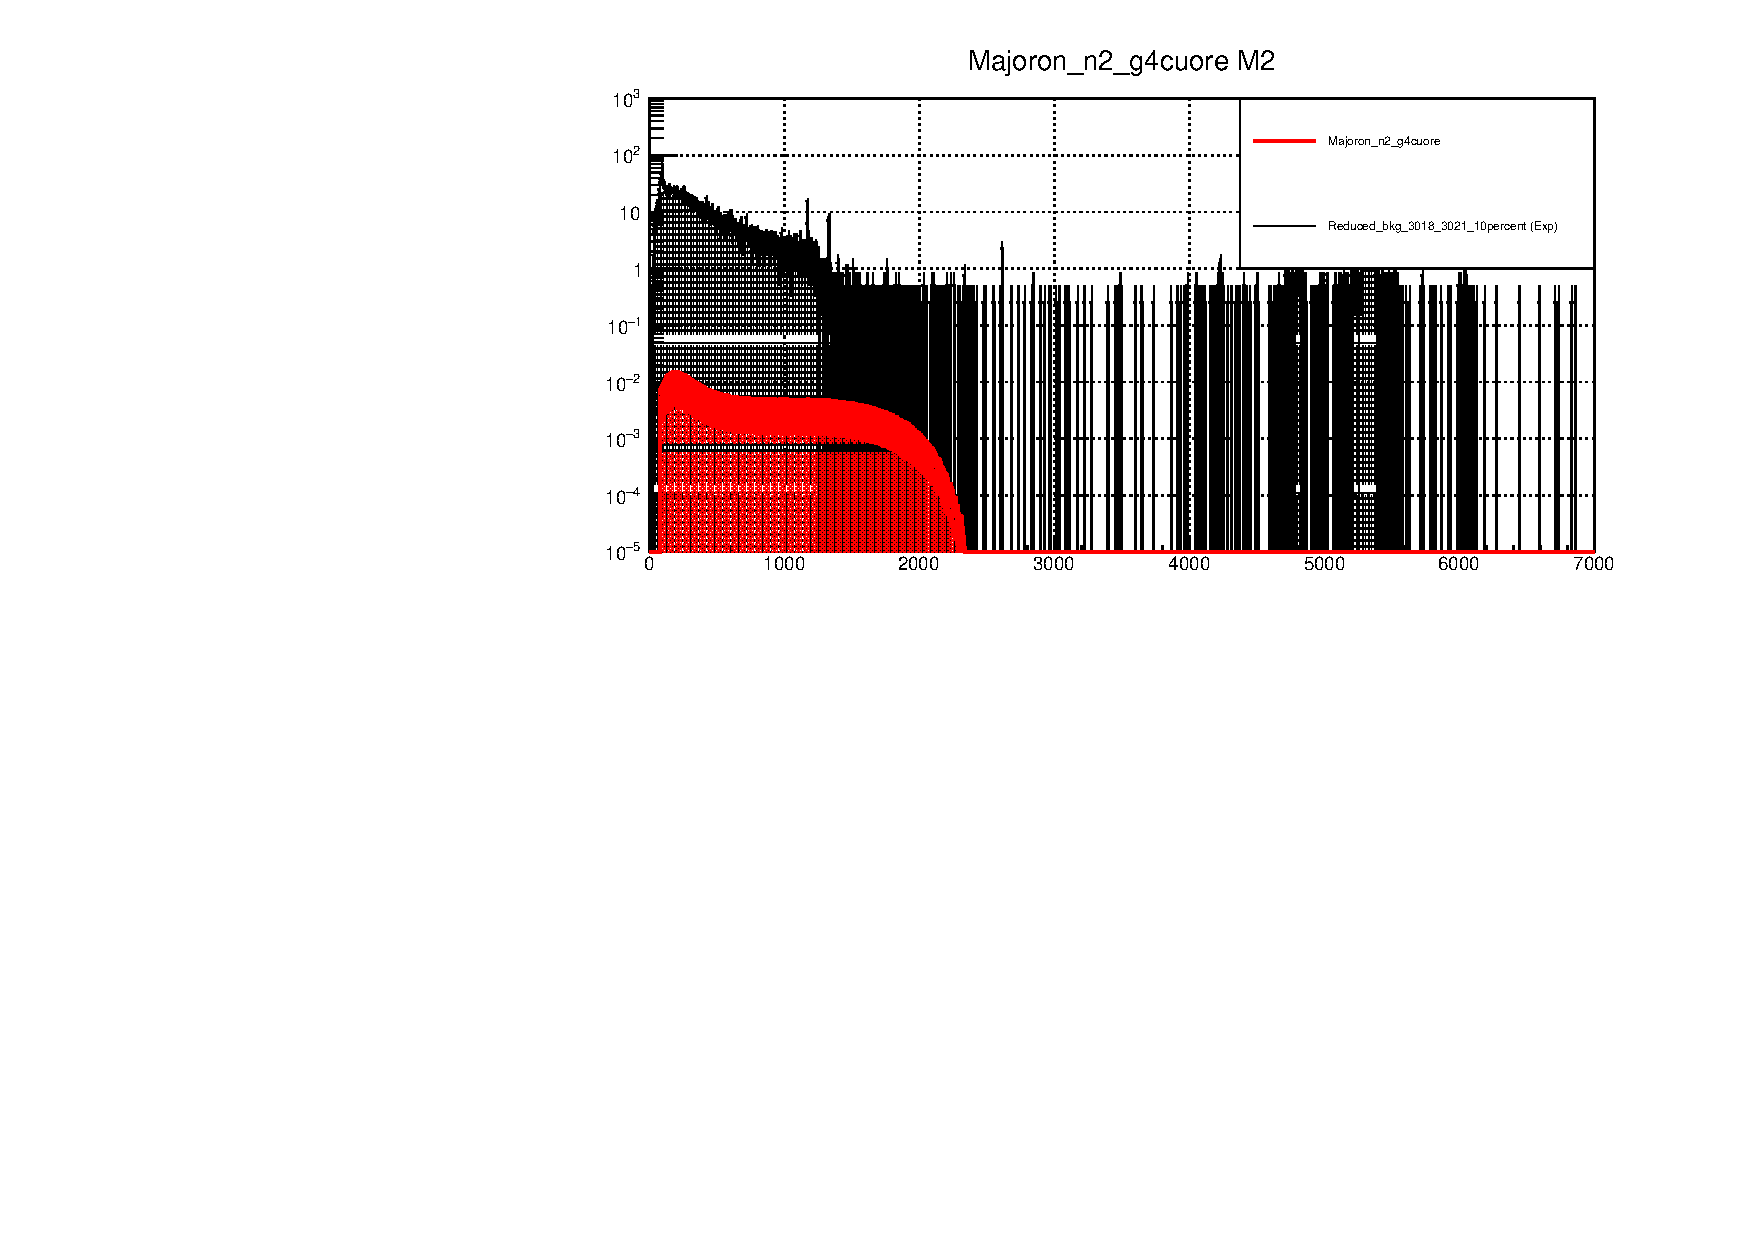
\includegraphics[width=0.9\textwidth]{Figures/Majoron_n2_g4cuore_M2.pdf}
\end{subfigure}
\qquad
\begin{subfigure}[t]{0.49\linewidth}
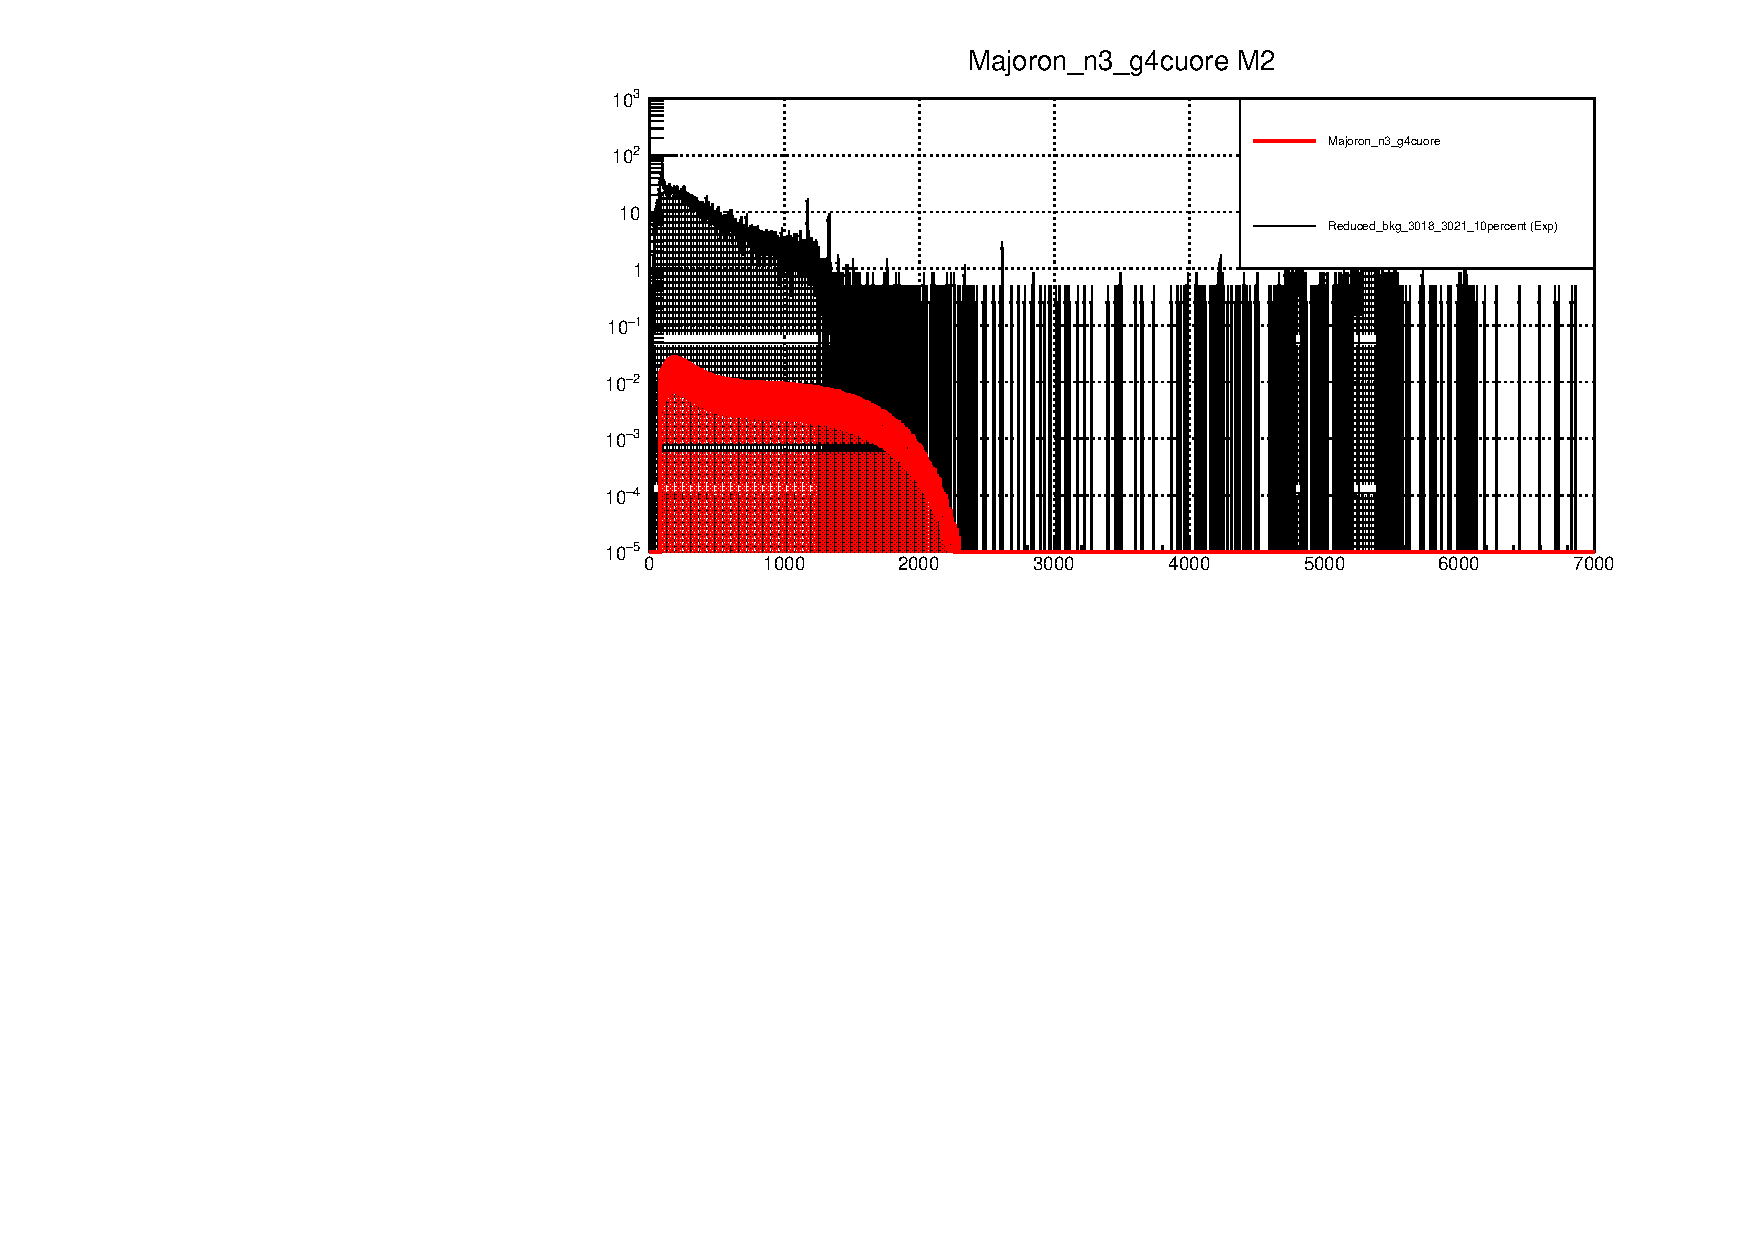
\includegraphics[width=0.9\textwidth]{Figures/Majoron_n3_g4cuore_M2.pdf}
\end{subfigure}
\qquad
\begin{subfigure}[t]{0.49\linewidth}
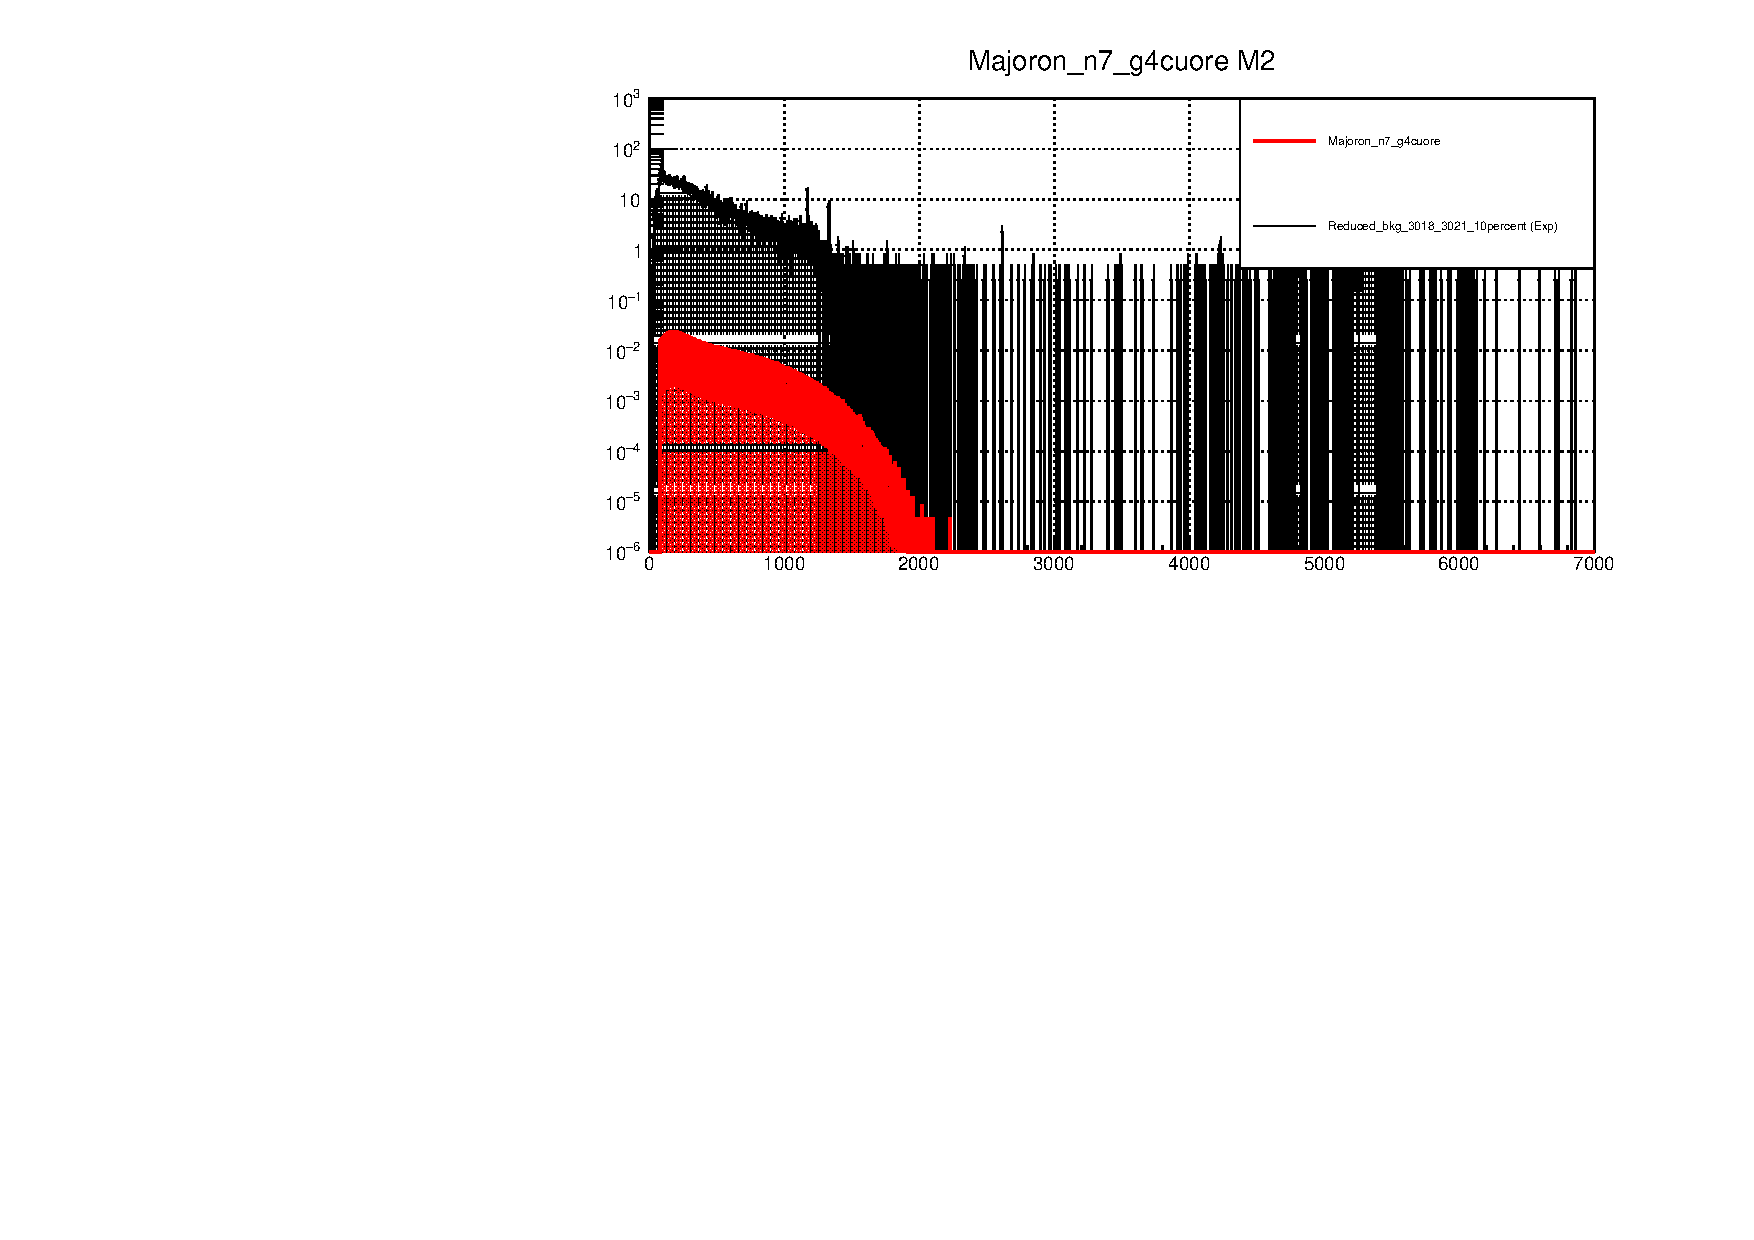
\includegraphics[width=0.9\textwidth]{Figures/Majoron_n7_g4cuore_M2.pdf}
\end{subfigure}
\caption[The fitted contribution of Majoron decays for the different spectral indices in the \Mtwo~ spectrum.]{The fitted contribution of Majoron decays for the different spectral indices in the \Mtwo~ spectrum.}
\label{fig:SpectralIndicesM2Fit}
\end{figure}

Figures to include: Correlation matrix, Fit value distributions for all the Majoron spectra, background model with only 2nu -- describe deficiencies i.e. alpha region low-E and 2 MeV, systematics (floors, layers, etc.), 